\documentclass[english,11pt,usenames,dvipsnames]{beamer}

\DeclareMathOperator{\Cov}{Cov}
\DeclareMathOperator{\Var}{Var}
\DeclareMathOperator{\E}{\mathbb{E}}
\DeclareMathOperator{\Proba}{\mathbb{P}}

\newcommand{\Covb}[2]{\ensuremath{\Cov\!\left[#1,#2\right]}}
\newcommand{\Eb}[1]{\ensuremath{\E\!\left[#1\right]}}
\newcommand{\Pb}[1]{\ensuremath{\Proba\!\left[#1\right]}}
\newcommand{\Varb}[1]{\ensuremath{\Var\!\left[#1\right]}}

% norm
\newcommand{\norm}[1]{\| #1 \|}

\newcommand{\indep}{\rotatebox[origin=c]{90}{$\models$}}





\usepackage{mathptmx,amsmath,amssymb,graphicx,bibentry,bbm,babel,ragged2e}

\makeatletter

\newcommand{\noun}[1]{\textsc{#1}}
\newcommand{\jitem}[1]{\item \begin{justify} #1 \end{justify} \vfill{}}
\newcommand{\sframe}[2]{\frame{\frametitle{#1} #2}}

\newenvironment{centercolumns}{\begin{columns}[c]}{\end{columns}}
%\newenvironment{jitem}{\begin{justify}\begin{itemize}}{\end{itemize}\end{justify}}

\usetheme{Warsaw}
\setbeamertemplate{footline}[text line]{}
\setbeamercolor{structure}{fg=purple!50!blue, bg=purple!50!blue}

\setbeamersize{text margin left=15pt,text margin right=15pt}

\setbeamercovered{transparent}

\setbeamertemplate{headline}{}
\setbeamertemplate{footline}[frame number]
\setbeamertemplate{navigation symbols}{}

\@ifundefined{showcaptionsetup}{}{%
 \PassOptionsToPackage{caption=false}{subfig}}
\usepackage{subfig}

\usepackage[utf8]{inputenc}
\usepackage[T1]{fontenc}


\usepackage{tikz}

\usepackage{multirow}


\usepackage{mdframed}

\usepackage[usenames,dvipsnames]{pstricks}
\usepackage{auto-pst-pdf}


\usepackage[dvipsnames]{xcolor}


\makeatother

\begin{document}


\title{Towards multi-scalar models for the co-evolution of transportation networks and territories}

\author{J.~Raimbault$^{1,2,3}$\\
\texttt{juste.raimbault@iscpif.fr}
}


\institute{$^{1}$UPS CNRS 3611 ISC-PIF\\
$^{2}$CASA, UCL\\
$^{3}$UMR CNRS 8504 G{\'e}ographie-cit{\'e}s
}


\date{Theo Quant 2019\\\smallskip
7 février 2019
}

\frame{\maketitle}

% Keywords: Transportation networks; Territories; Co-evolution; Modeling; Multi-scale

% plan :
%   - co-evolution : difficult issues
%   - recall previous results
%   - describe model with physical nw (heuristic, synthetic setup etc)
%.  - perspective : describe multi-scalar avec mesocoevol (two entries into multiscalar : "top-down" (precise a macro model) ; "bottom-up" (inserting meso instances into a macro coupling structure.



\section{Introduction}


\sframe{Interactions between networks and territories}{

%The intricate relations between transportation networks and territories, at multiples scales, has fed numerous open questions such as the potential existence of structuring effects of networks \cite{offner1993effets}.

% striking example for Besac.

\centering

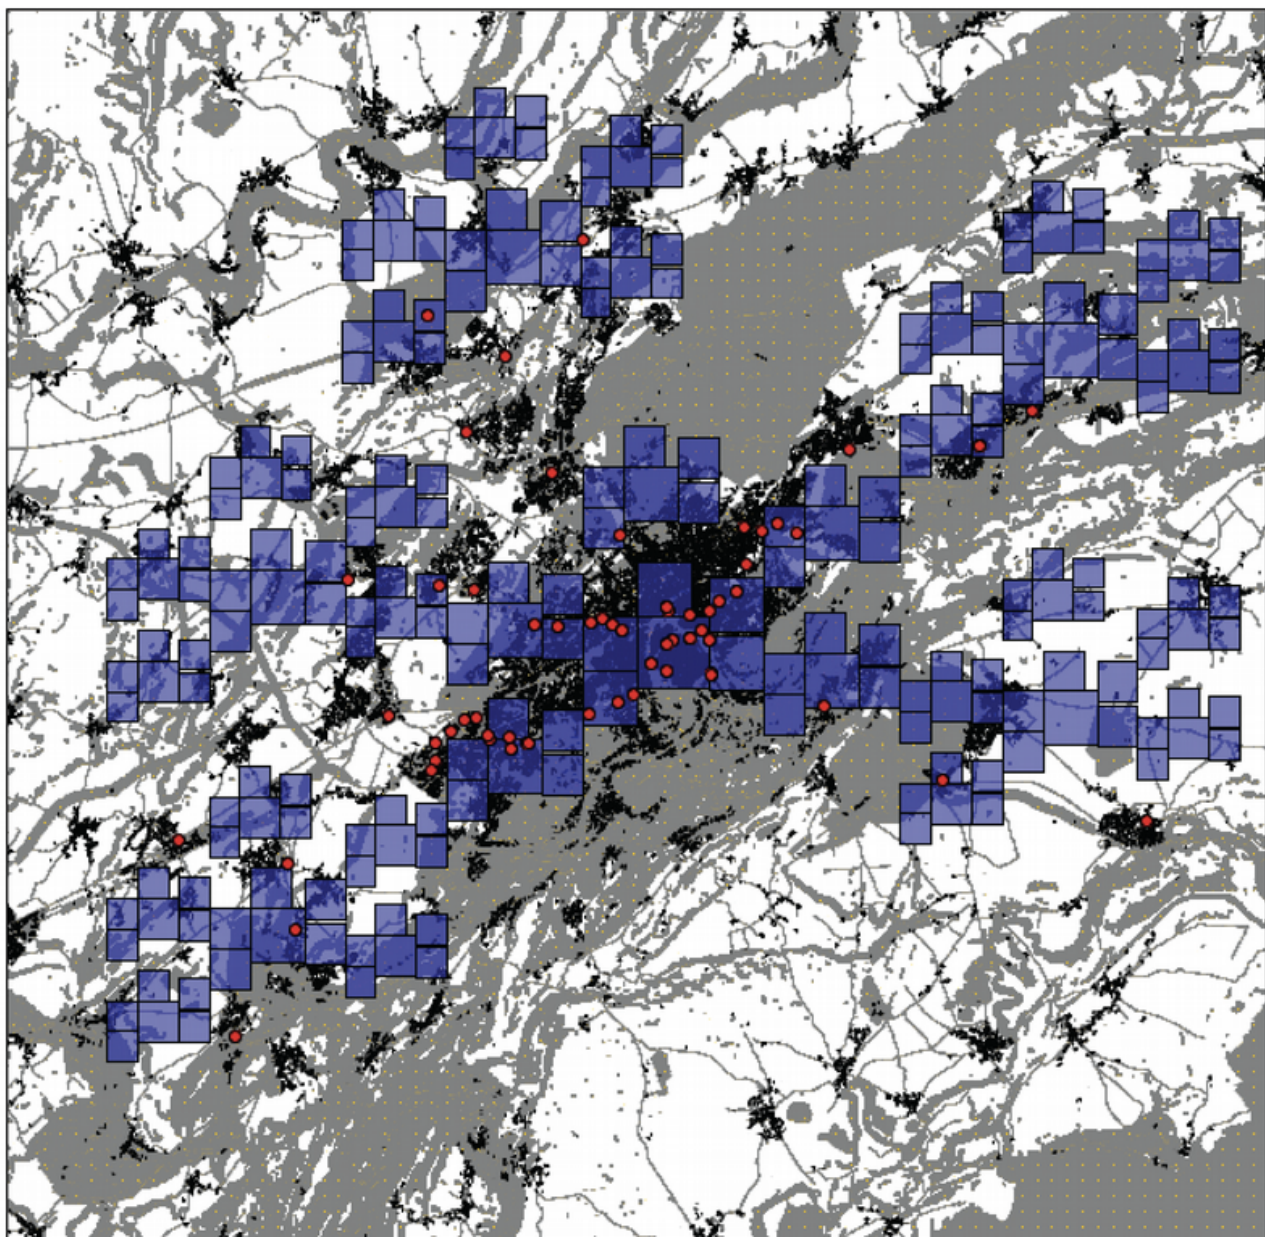
\includegraphics[height=0.7\textheight]{figures/fractalopolis.png}

\cite{tannier:tel-01668615}


}



\sframe{Modeling the co-evolution of transportation networks and territories}{
 
 % \cite{raimbault2018caracterisation} explored these interactions from the point of view of co-evolutive dynamics, aiming at modeling these. In particular, \cite{raimbault2018modeling} introduced a co-evolution model at the macroscopic scale for systems of cities with abstract networks, whereas \cite{raimbault2018urban} developed a morphogenesis model at the mesoscopic scale, capturing the co-evolution between road networks and the population density grid.
 
}



\sframe{Towards multi-scalar models}{

% The processes included in models depend naturally on the scale. This communication aims at showing the necessity of a multi-scalar approach for a more accurate account of these co-evolutive dynamics.


}


\sframe{Generic description of the model}{

% We introduce first a physical implementation of transportation networks into the macroscopic model, with a description of networks with a 1km spatial resolution, whereas the typical range of application of the model is around 1000km.



\centering

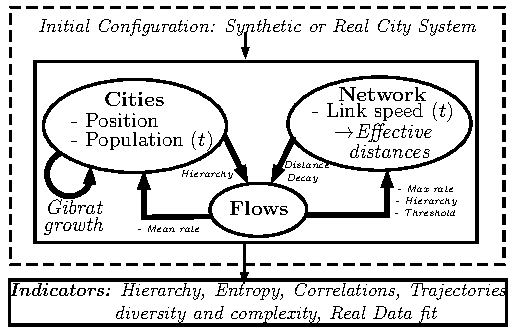
\includegraphics[width=\textwidth]{figures/model.pdf}

}



\sframe{Physical network specification}{

}


\sframe{Synthetic physical network}{

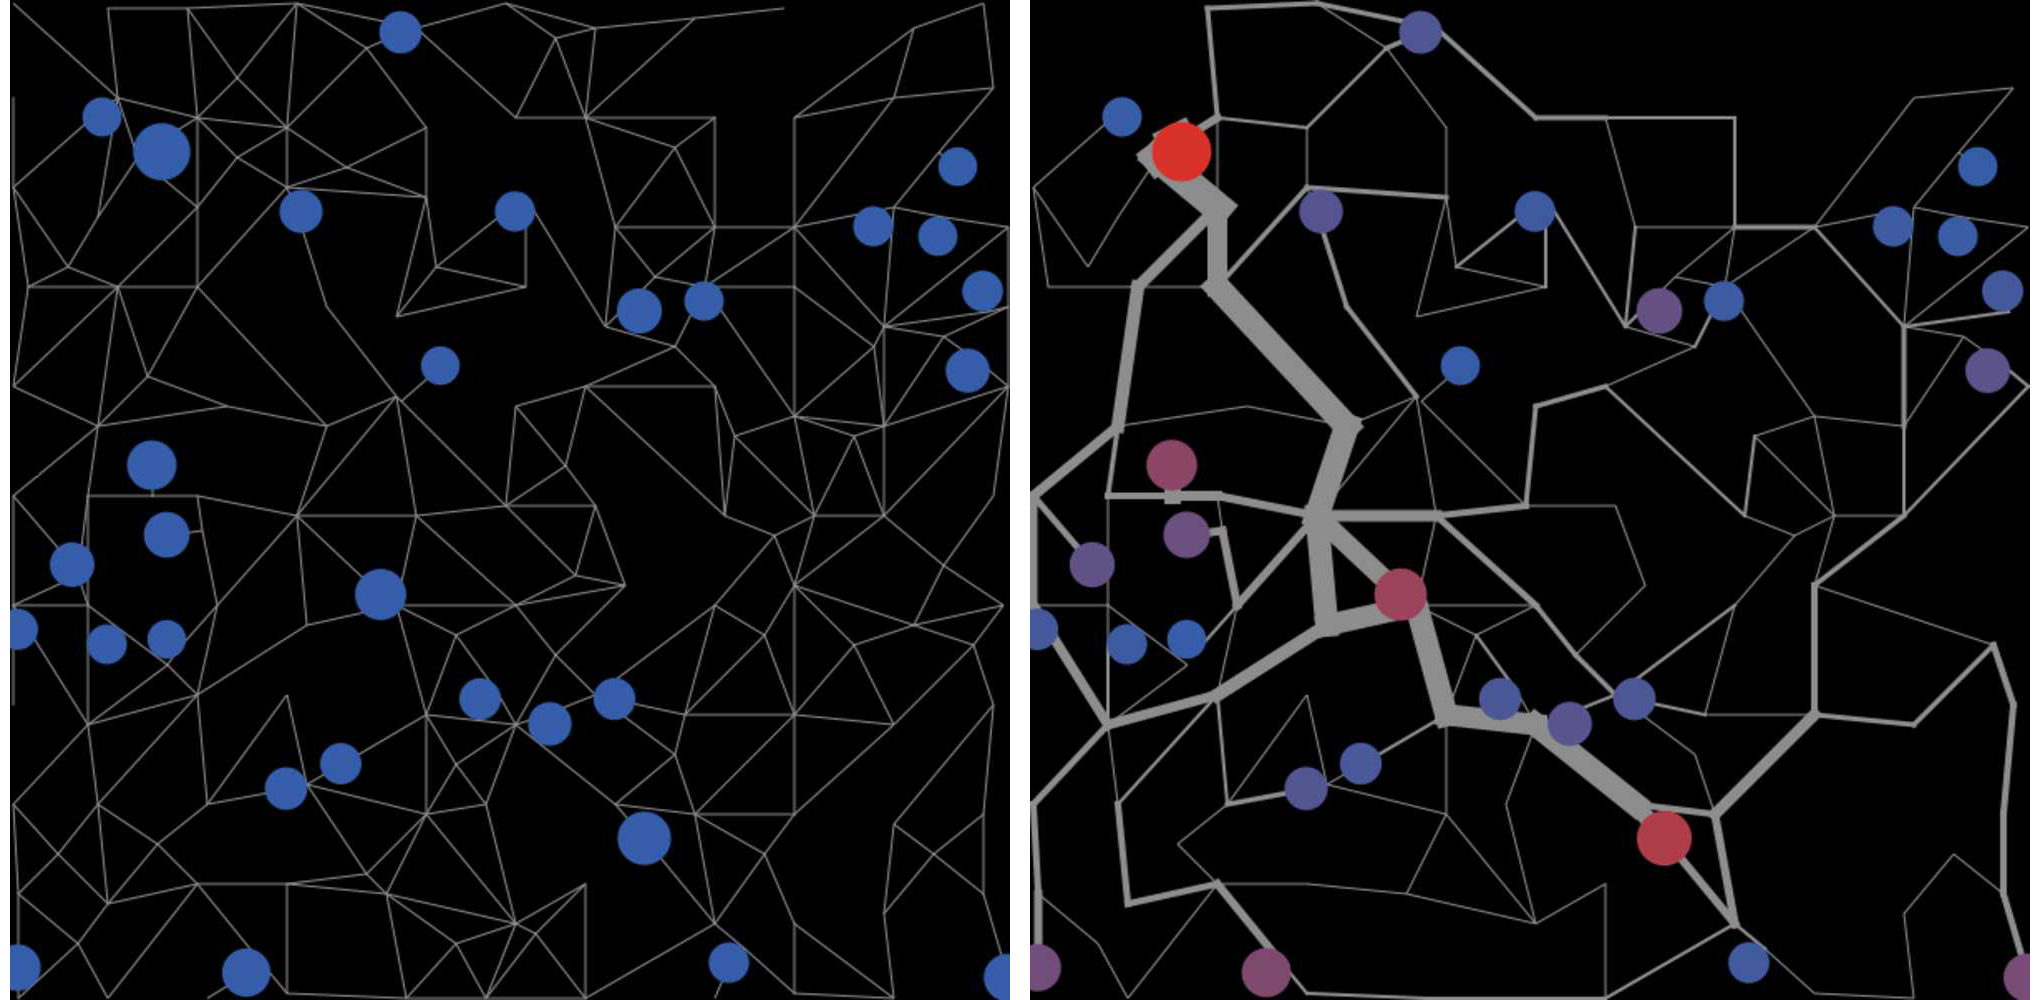
\includegraphics[width=\textwidth]{figures/6-2-3-fig-macrocoevol-slimemould.jpg}

}


\sframe{Model calibration}{

% Calibrations are done for different versions of each model including more or less parameters, using distributed genetic algorithms on a computation grid through the intermediary of the OpenMOLE model exploration software [6]. 

Bi-objective calibration of 7 models for 7 city systems $\rightarrow$ use of genetic algorithms on grid, made smooth with the OpenMOLE software \url{https://next.openmole.org/}

\centering

\smallskip


\includegraphics[height=0.35\textheight]{figures/openmole.png}

\smallskip

\raggedright\justify

\footnotesize \textit{OpenMOLE: (i) embed any model as a black box; (ii) transparent access to main High Performance Computing environments; (iii) model exploration and calibration methods.}

\bigskip

\textbf{Come to the Satellite on Wednesday, and apply to the summer school !} 
\\(\texttt{https://exmodelo.org/})

}


\sframe{Model behavior}{

% Systematic explorations of the model on synthetic data using the OpenMole software show that even with the same processes for network growth, qualitative behavior fundamentally differ.
% -> OK ; ex no existence of the complexity maximum

\begin{columns}
	\begin{column}{0.5\linewidth}
		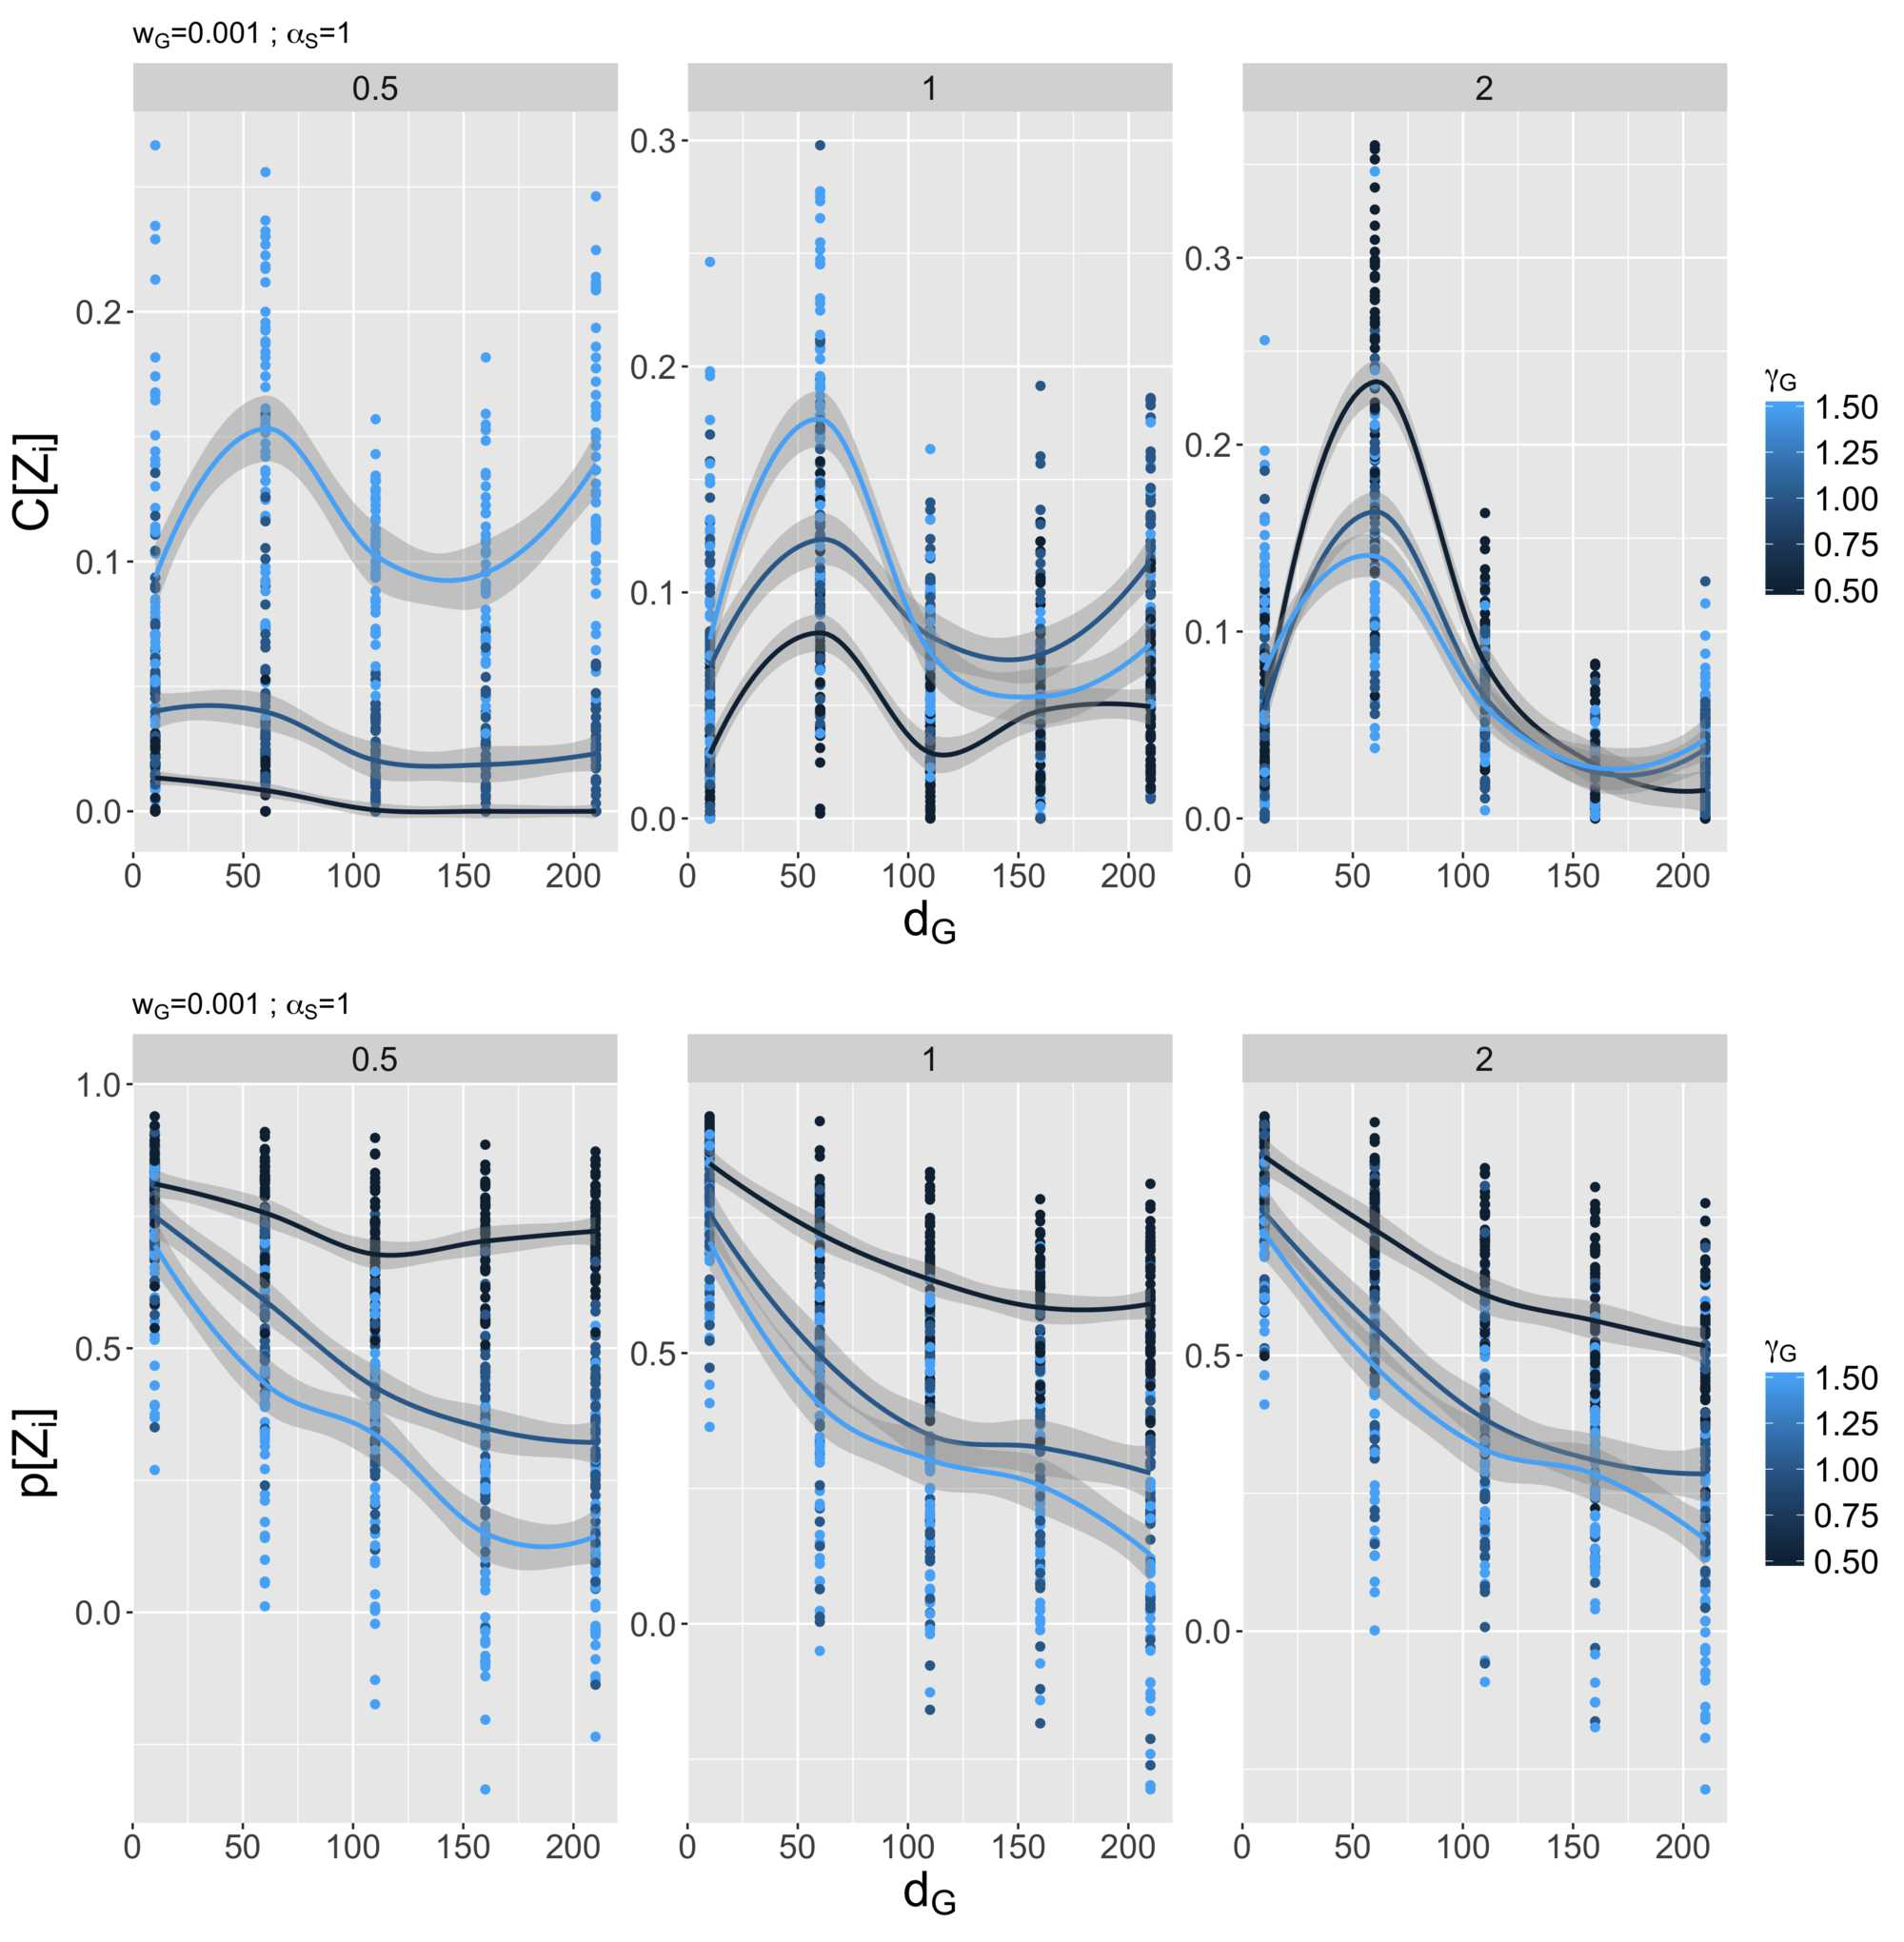
\includegraphics[width=\textwidth]{figures/6-2-2-fig-macrocoevol-behavior-aggreg.jpg}
	\end{column}
	\begin{column}{0.5\linewidth}
		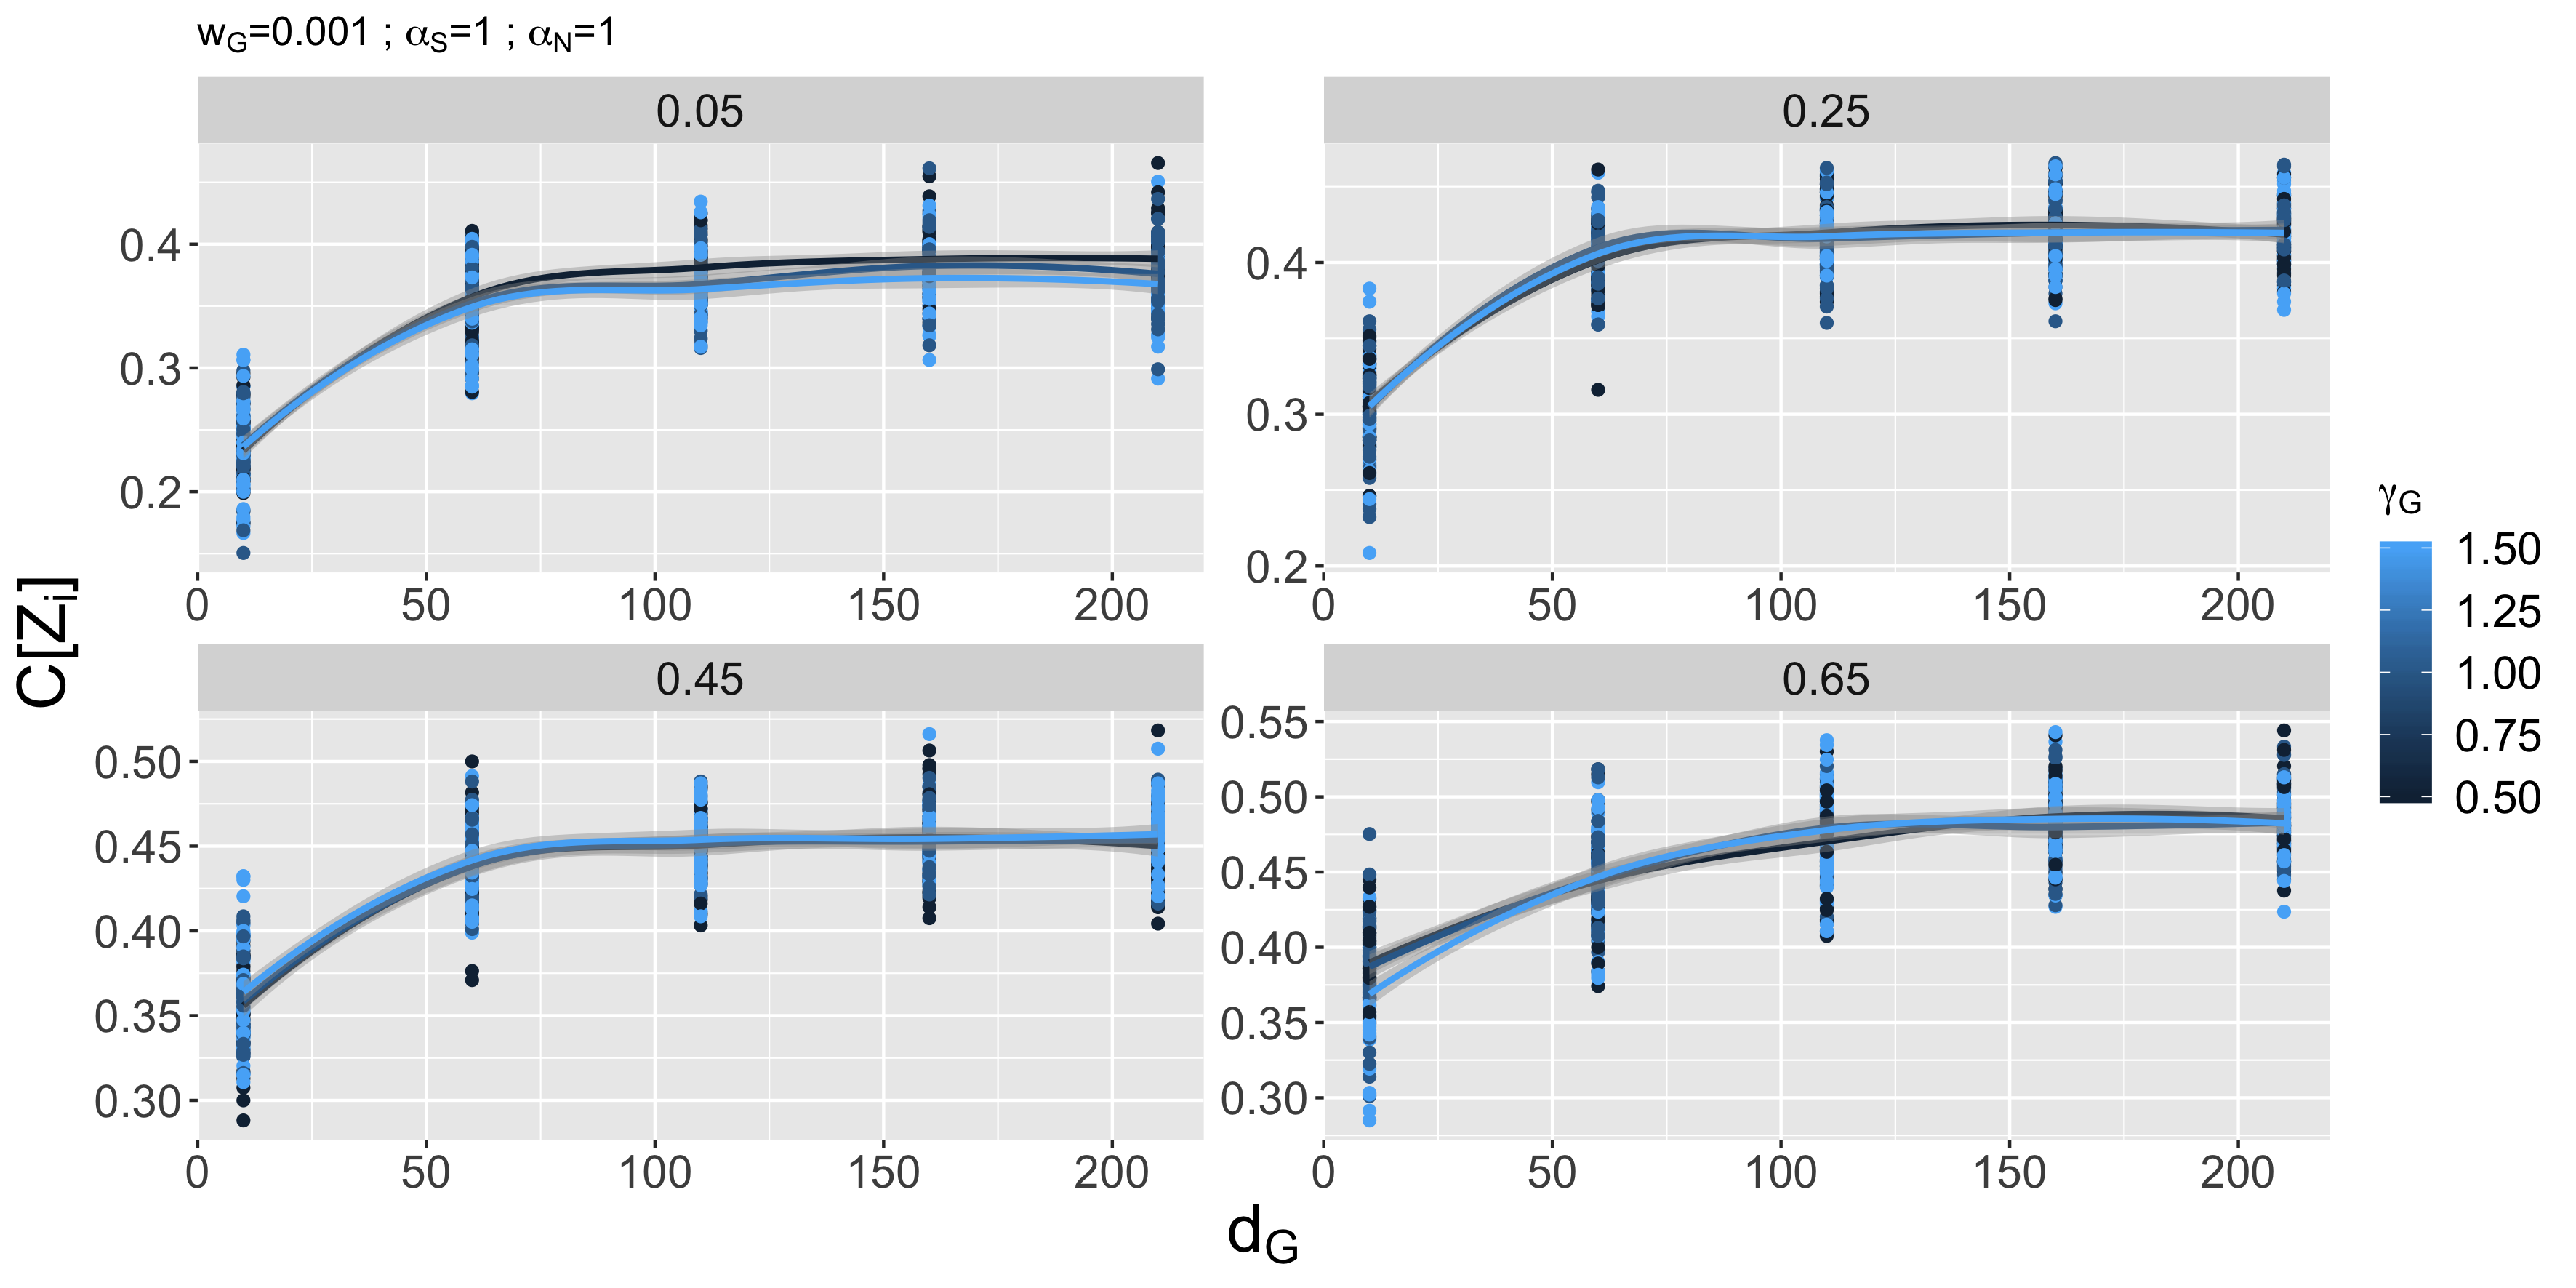
\includegraphics[width=\textwidth]{figures/complexityAccessibility_synthrankSize1_nwGmax0_05_gravityWeight0_001_nwExponent1.png}\\
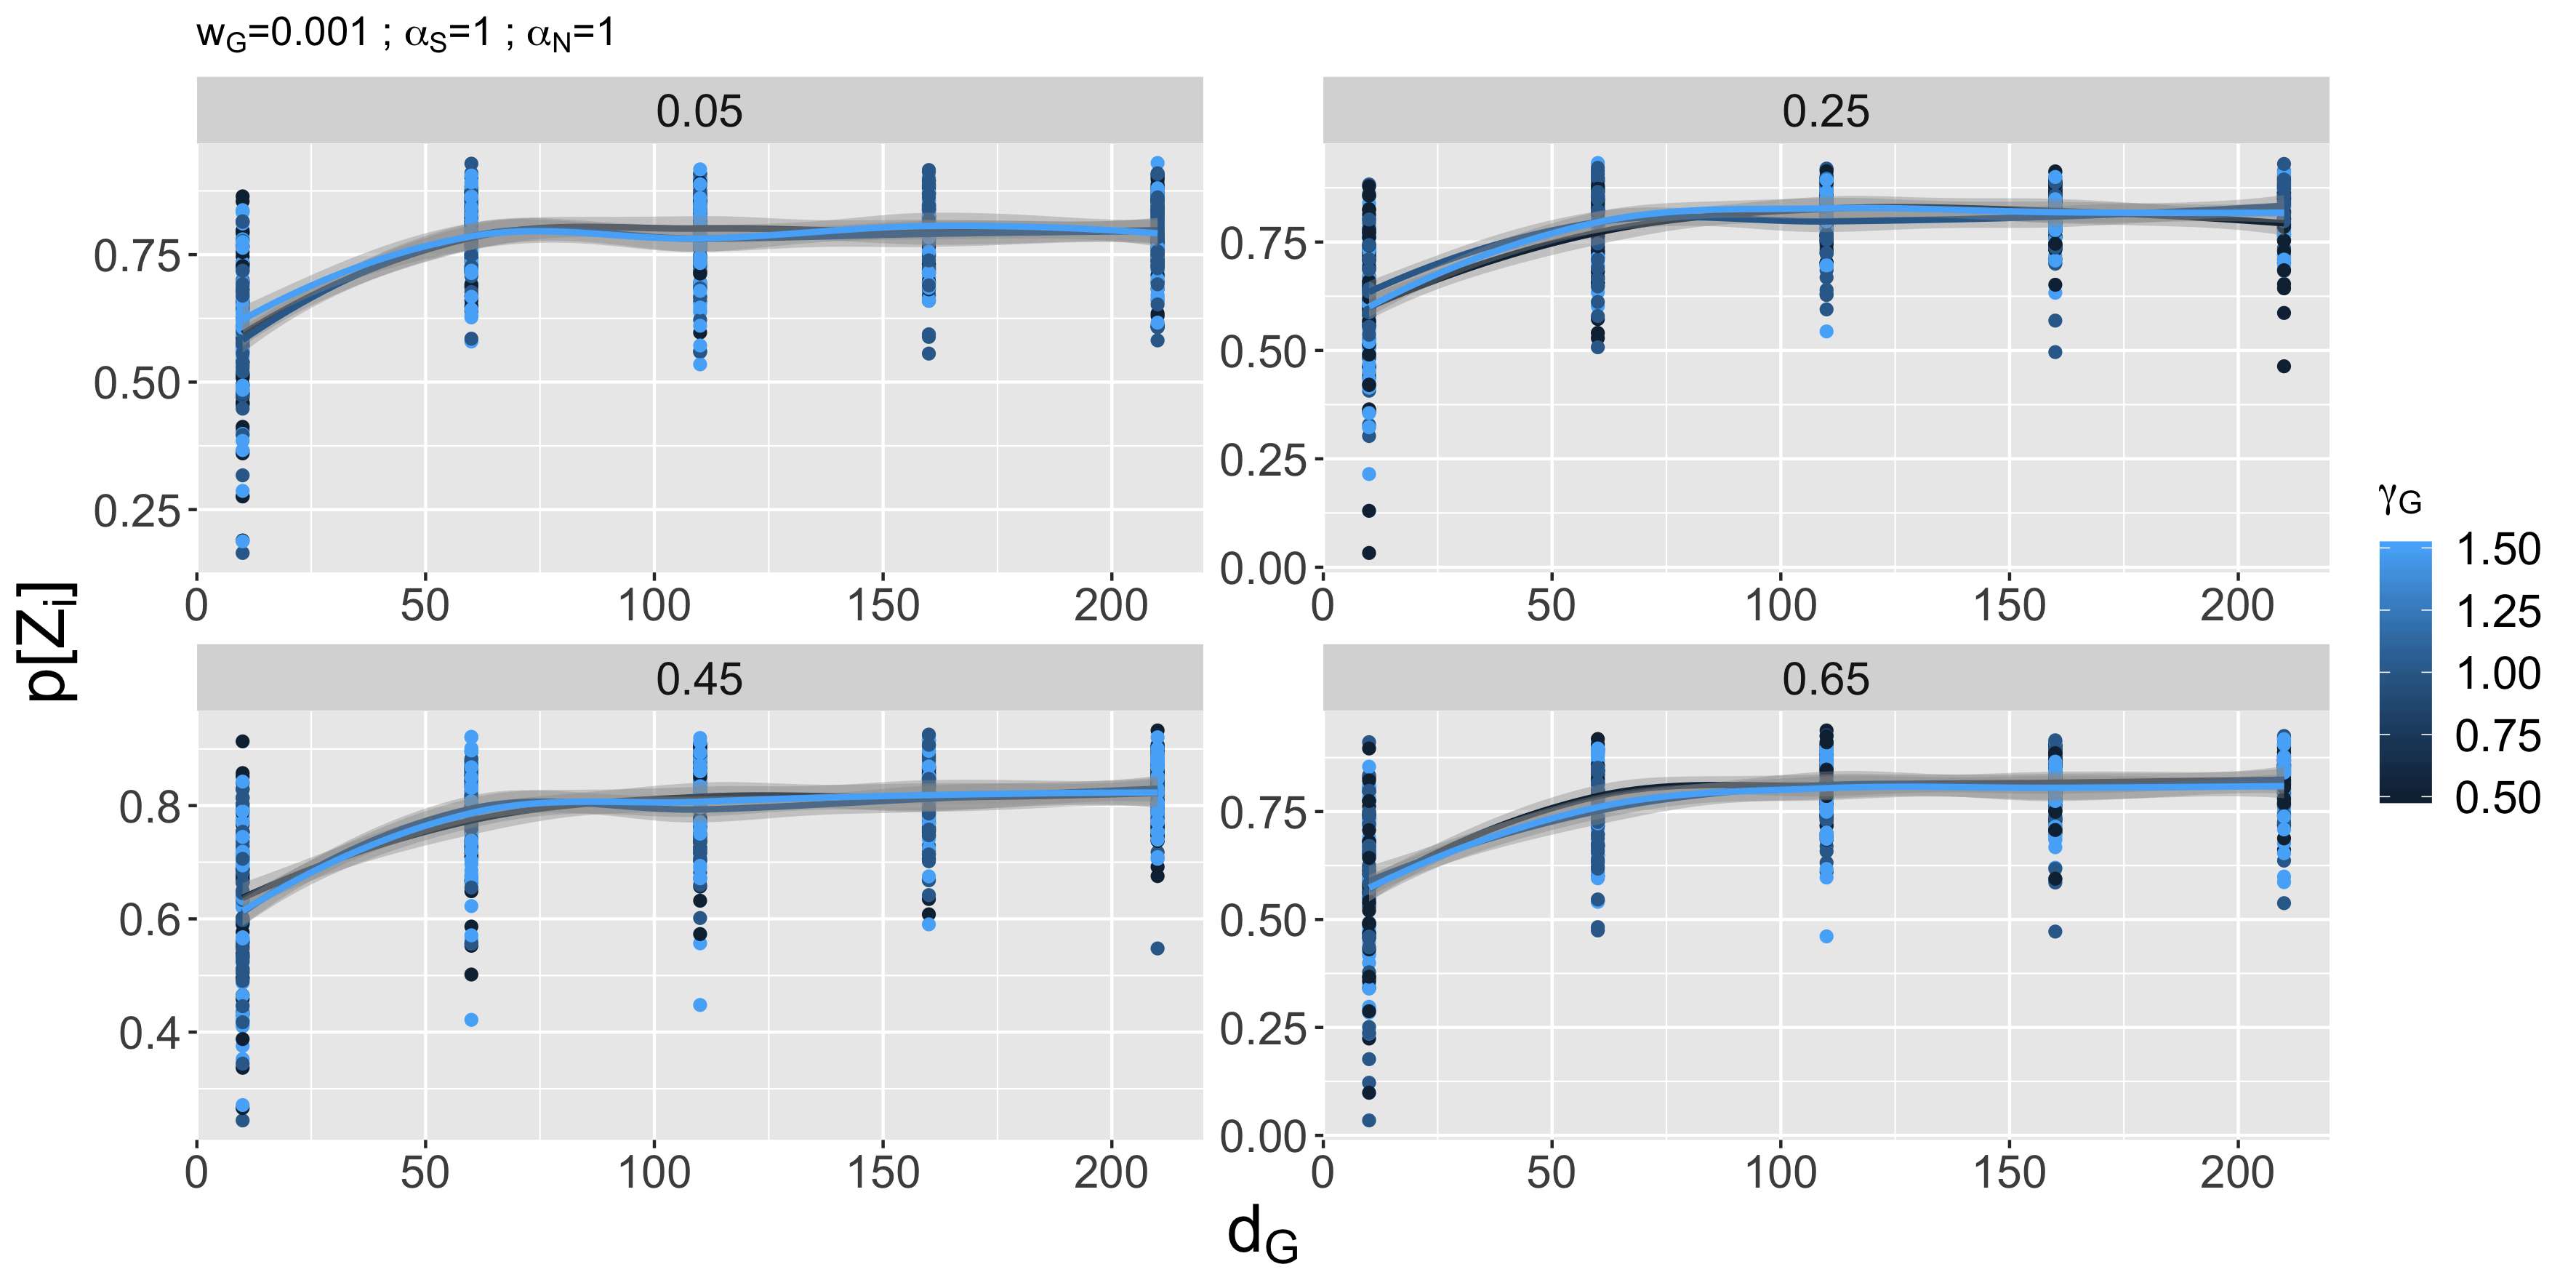
\includegraphics[width=\textwidth]{figures/rankCorrAccessibility_synthrankSize1_nwGmax0_05_gravityWeight0_001_nwExponent1.png}
	\end{column}
\end{columns}


}


\sframe{Interaction regimes}{

%  In particular, co-evolutive dynamics are more difficult to characterize in the hybrid scale models, recalling results obtained by \cite{raimbault2018caracterisation} with the SimpopNet model \cite{schmitt2014modelisation} which has a similar structure.
% -> seems less with grid explo ; may be difficult to say in general (-> PSE needed)

% number of regimes 




}


\sframe{Model calibration}{

% Calibration on the French system of cities with the objective of population and distance matrices accurateness gives mitigated results in comparison to the original model, but however witnesses fit improvement on several temporal calibration windows. These results suggest that the hybrid model would be closer to the actual complexity of these dynamics, as it was shown by \cite{raimbault2018modeling} that co-evolution is indeed difficult to characterize empirically for the French system of cities with railway network data.

% - more constrained physical model ? (rq : no link creation -> the hardest part is still left behind - should couple with an effective network growth model ? )
% - rq : much much better results for abstract flows : few evolutions, do not accurately reflected by flow reinforcement.
% - why so few points on the Pareto front ?


}


\sframe{Theoretical proposal for a multi-scalar model}{

%   We finally discuss from a theoretical point of view what would be the advantages of a multi-scale coupling of the macroscopic and the mesoscopic model (including for example a more operational character, more accurate conditioning of local dynamics by exogenous parameters determined at the macroscopic scale, a better grasp on spatio-temporal non-stationarity) and present different modeling alternatives that could be followed to achieve this coupling.


}




\sframe{Discussion}{

\justify

\textit{Developments}

\bigskip

% cf simpopnet chapter
$\rightarrow$ fair comparison of number of regimes using PSE algorithm 

\bigskip

$\rightarrow$ 


}




\section{Conclusion}


\sframe{Conclusion}{

\justify

\small

$\rightarrow$ 
%Vers une intégration plus systématique (épistémologiquement et théoriquement) des différentes complexités pour l'étude des systèmes territoriaux ? \\\cite{raimbault2018relating}

\medskip

$\rightarrow$ 
%Réflexivité (entre autre complexité appliquée à la complexité) nécessaire pour une connaissance complexe \cite{morin1991methode} ; vers un perspectivisme appliqué ? \cite{banos2018spatialised}

\bigskip

\footnotesize

\textbf{References}

Raimbault, J. (2018). Calibration of a density-based model of urban morphogenesis. PloS one, 13(9):e0203516

\smallskip

Raimbault, J. (2019). An Urban Morphogenesis Model Capturing Interactions Between Networks and Territories. In L. D'Acci (ed.), The Mathematics of Urban Morphology. Springer Nature Switzerland AG.

\smallskip

Raimbault, J. (2018). Indirect evidence of network effects in a system of cities. Environment and Planning B: Urban Analytics and City Science, 2399808318774335.

\smallskip

Raimbault, J. (2019). Modeling the co-evolution of cities and networks. Forthcoming in Handbook of Cities and Networks, Rozenblat C., Niel Z. (eds.), Edward Elgar Publishing.

\smallskip

Raimbault, J., Banos, A., \& Doursat, R. (2014, June). A Hybrid Network/Grid Model of Urban Morphogenesis and Optimization. In 4th International Conference on Complex Systems and Applications (pp. 51-60).

\bigskip


% + dataverse
\footnotesize{ - Code, data and results\\ \texttt{https://github.com/JusteRaimbault/CoevolutionNwTerritories}\\
- Acknowledgements to the \textit{European Grid Infrastructure} and its \textit{National Grid Initiatives} (\textit{France-Grilles} in particular) for the technical support and the infrastructure.

}

}








%%%%%%%%%%%%%%%%%%%%%
\begin{frame}[allowframebreaks]
\frametitle{References}
\bibliographystyle{apalike}
\bibliography{biblio}
\end{frame}
%%%%%%%%%%%%%%%%%%%%%%%%%%%%










\end{document}







